\documentclass[]{article}
\usepackage{lmodern}
\usepackage{amssymb,amsmath}
\usepackage{ifxetex,ifluatex}
\usepackage{fixltx2e} % provides \textsubscript
\ifnum 0\ifxetex 1\fi\ifluatex 1\fi=0 % if pdftex
  \usepackage[T1]{fontenc}
  \usepackage[utf8]{inputenc}
\else % if luatex or xelatex
  \ifxetex
    \usepackage{mathspec}
    \usepackage{xltxtra,xunicode}
  \else
    \usepackage{fontspec}
  \fi
  \defaultfontfeatures{Mapping=tex-text,Scale=MatchLowercase}
  \newcommand{\euro}{€}
\fi
% use upquote if available, for straight quotes in verbatim environments
\IfFileExists{upquote.sty}{\usepackage{upquote}}{}
% use microtype if available
\IfFileExists{microtype.sty}{\usepackage{microtype}}{}
\usepackage[margin=1in]{geometry}
\usepackage{color}
\usepackage{fancyvrb}
\newcommand{\VerbBar}{|}
\newcommand{\VERB}{\Verb[commandchars=\\\{\}]}
\DefineVerbatimEnvironment{Highlighting}{Verbatim}{commandchars=\\\{\}}
% Add ',fontsize=\small' for more characters per line
\newenvironment{Shaded}{}{}
\newcommand{\AlertTok}[1]{\textcolor[rgb]{1.00,0.00,0.00}{\textbf{#1}}}
\newcommand{\AnnotationTok}[1]{\textcolor[rgb]{0.38,0.63,0.69}{\textbf{\textit{#1}}}}
\newcommand{\AttributeTok}[1]{\textcolor[rgb]{0.49,0.56,0.16}{#1}}
\newcommand{\BaseNTok}[1]{\textcolor[rgb]{0.25,0.63,0.44}{#1}}
\newcommand{\BuiltInTok}[1]{#1}
\newcommand{\CharTok}[1]{\textcolor[rgb]{0.25,0.44,0.63}{#1}}
\newcommand{\CommentTok}[1]{\textcolor[rgb]{0.38,0.63,0.69}{\textit{#1}}}
\newcommand{\CommentVarTok}[1]{\textcolor[rgb]{0.38,0.63,0.69}{\textbf{\textit{#1}}}}
\newcommand{\ConstantTok}[1]{\textcolor[rgb]{0.53,0.00,0.00}{#1}}
\newcommand{\ControlFlowTok}[1]{\textcolor[rgb]{0.00,0.44,0.13}{\textbf{#1}}}
\newcommand{\DataTypeTok}[1]{\textcolor[rgb]{0.56,0.13,0.00}{#1}}
\newcommand{\DecValTok}[1]{\textcolor[rgb]{0.25,0.63,0.44}{#1}}
\newcommand{\DocumentationTok}[1]{\textcolor[rgb]{0.73,0.13,0.13}{\textit{#1}}}
\newcommand{\ErrorTok}[1]{\textcolor[rgb]{1.00,0.00,0.00}{\textbf{#1}}}
\newcommand{\ExtensionTok}[1]{#1}
\newcommand{\FloatTok}[1]{\textcolor[rgb]{0.25,0.63,0.44}{#1}}
\newcommand{\FunctionTok}[1]{\textcolor[rgb]{0.02,0.16,0.49}{#1}}
\newcommand{\ImportTok}[1]{#1}
\newcommand{\InformationTok}[1]{\textcolor[rgb]{0.38,0.63,0.69}{\textbf{\textit{#1}}}}
\newcommand{\KeywordTok}[1]{\textcolor[rgb]{0.00,0.44,0.13}{\textbf{#1}}}
\newcommand{\NormalTok}[1]{#1}
\newcommand{\OperatorTok}[1]{\textcolor[rgb]{0.40,0.40,0.40}{#1}}
\newcommand{\OtherTok}[1]{\textcolor[rgb]{0.00,0.44,0.13}{#1}}
\newcommand{\PreprocessorTok}[1]{\textcolor[rgb]{0.74,0.48,0.00}{#1}}
\newcommand{\RegionMarkerTok}[1]{#1}
\newcommand{\SpecialCharTok}[1]{\textcolor[rgb]{0.25,0.44,0.63}{#1}}
\newcommand{\SpecialStringTok}[1]{\textcolor[rgb]{0.73,0.40,0.53}{#1}}
\newcommand{\StringTok}[1]{\textcolor[rgb]{0.25,0.44,0.63}{#1}}
\newcommand{\VariableTok}[1]{\textcolor[rgb]{0.10,0.09,0.49}{#1}}
\newcommand{\VerbatimStringTok}[1]{\textcolor[rgb]{0.25,0.44,0.63}{#1}}
\newcommand{\WarningTok}[1]{\textcolor[rgb]{0.38,0.63,0.69}{\textbf{\textit{#1}}}}
\usepackage{graphicx}
\makeatletter
\def\maxwidth{\ifdim\Gin@nat@width>\linewidth\linewidth\else\Gin@nat@width\fi}
\def\maxheight{\ifdim\Gin@nat@height>\textheight\textheight\else\Gin@nat@height\fi}
\makeatother
% Scale images if necessary, so that they will not overflow the page
% margins by default, and it is still possible to overwrite the defaults
% using explicit options in \includegraphics[width, height, ...]{}
\setkeys{Gin}{width=\maxwidth,height=\maxheight,keepaspectratio}
\ifxetex
  \usepackage[setpagesize=false, % page size defined by xetex
              unicode=false, % unicode breaks when used with xetex
              xetex]{hyperref}
\else
  \usepackage[unicode=true]{hyperref}
\fi
\hypersetup{breaklinks=true,
            bookmarks=true,
            pdfauthor={Justin Le},
            pdftitle={A Purely Functional Typed Approach to Trainable Models (Part 2)},
            colorlinks=true,
            citecolor=blue,
            urlcolor=blue,
            linkcolor=magenta,
            pdfborder={0 0 0}}
\urlstyle{same}  % don't use monospace font for urls
% Make links footnotes instead of hotlinks:
\renewcommand{\href}[2]{#2\footnote{\url{#1}}}
\setlength{\parindent}{0pt}
\setlength{\parskip}{6pt plus 2pt minus 1pt}
\setlength{\emergencystretch}{3em}  % prevent overfull lines
\setcounter{secnumdepth}{0}

\title{A Purely Functional Typed Approach to Trainable Models (Part 2)}
\author{Justin Le}
\date{May 14, 2018}

\begin{document}
\maketitle

\emph{Originally posted on
\textbf{\href{https://blog.jle.im/entry/purely-functional-typed-models-2.html}{in
Code}}.}

Welcome back! We're going to be jumping right back into describing a vision of a
purely functional typed approach to writing trainable models using
differentiable programming. If you're just joining us, be sure to check out
\href{https://blog.jle.im/entry/purely-functional-typed-models-1.html}{Part 1}
first!

In the last post, we looked at models as ``question and answer'' systems. We
described them as essentially being functions of type

{[} f : P \textbackslash{}rightarrow (A \textbackslash{}rightarrow
B){]}(https://latex.codecogs.com/png.latex?\%0Af\%20\%3A\%20P\%20\%5Crightarrow\%20\%28A\%20\%5Crightarrow\%20B\%29\%0A
" f : P \rightarrow (A \rightarrow B) ``)

Where, for
\includegraphics{https://latex.codecogs.com/png.latex?f_p\%28x\%29\%20\%3D\%20y},
you have a ``question''
\includegraphics{https://latex.codecogs.com/png.latex?x\%20\%3A\%20A} and are
looking for an ``answer''
\includegraphics{https://latex.codecogs.com/png.latex?y\%20\%3A\%20B}. Picking a
\emph{different}
\includegraphics{https://latex.codecogs.com/png.latex?p\%20\%3A\%20P} will give
a \emph{different}
\includegraphics{https://latex.codecogs.com/png.latex?A\%20\%5Crightarrow\%20B}
function. We claimed that training a model was finding just the right
\includegraphics{https://latex.codecogs.com/png.latex?p} to use with the model
to yield the right
\includegraphics{https://latex.codecogs.com/png.latex?A\%20\%5Crightarrow\%20B}
function that models your situation.

We then noted that if you have a set of \texttt{(a,\ b)} observations, and your
function is differentiable, you can find the \emph{gradient} of \texttt{p} with
respect to the error of your model on each observation, which tells you how to
nudge a given \texttt{p} in order to reduce how wrong your model is for that
observation. By repeatedly making observations and taking those nudges, you can
arrive at a suitable \texttt{p} to model any situation.

This is great if we consider a model as ``question and answer'', but sometimes
things don't fit so cleanly. Today, we're going to be looking at a whole
different type of model (``time series'' models) and see how they are different,
but also how they are really the same.

\hypertarget{time-series-models}{%
\section{Time Series Models}\label{time-series-models}}

In the wild, many models are not simple ``question and answer'', but rather
represent a ``time series''. As a generalization, we can talk about time series
models as:

{[} f\_p(x,t) =
y{]}(https://latex.codecogs.com/png.latex?\%0Af\_p\%28x\%2Ct\%29\%20\%3D\%20y\%0A
" f\_p(x,t) = y ``)

Which says, given an input and a time, return an output based on both. The point
of this is to let us have recurrent relationships, like for
\href{https://en.wikipedia.org/wiki/Autoregressive_model}{autoregressive models}
found in statistics:

{[} \textbackslash{}text\{AR\}\_\{\textbackslash{}phi\_1,
\textbackslash{}phi\_2, \textbackslash{}ldots\}(x,t) =
\textbackslash{}epsilon\_t + \textbackslash{}phi\_1
\textbackslash{}text\{AR\}\_\{\textbackslash{}phi\_1, \textbackslash{}phi\_2,
\textbackslash{}ldots\}(x, t-1) + \textbackslash{}phi\_2
\textbackslash{}text\{AR\}\_\{\textbackslash{}phi\_1, \textbackslash{}phi\_2,
\textbackslash{}ldots\}(x, t-2) +
\textbackslash{}ldots{]}(https://latex.codecogs.com/png.latex?\%0A\%5Ctext\%7BAR\%7D\_\%7B\%5Cphi\_1\%2C\%20\%5Cphi\_2\%2C\%20\%5Cldots\%7D\%28x\%2Ct\%29\%0A\%20\%20\%3D\%20\%5Cepsilon\_t\%20\%2B\%20\%5Cphi\_1\%20\%5Ctext\%7BAR\%7D\_\%7B\%5Cphi\_1\%2C\%20\%5Cphi\_2\%2C\%20\%5Cldots\%7D\%28x\%2C\%20t-1\%29\%0A\%20\%20\%2B\%20\%5Cphi\_2\%20\%5Ctext\%7BAR\%7D\_\%7B\%5Cphi\_1\%2C\%20\%5Cphi\_2\%2C\%20\%5Cldots\%7D\%28x\%2C\%20t-2\%29\%0A\%20\%20\%2B\%20\%5Cldots\%0A
" \text{AR}\_\{\phi\_1, \phi\_2, \ldots\}(x,t) = \epsilon\_t + \phi\emph{1
\text{AR}}\{\phi\_1, \phi\_2, \ldots\}(x, t-1) + \phi\emph{2
\text{AR}}\{\phi\_1, \phi\_2, \ldots\}(x, t-2) + \ldots ``)

However, this is a bad way of \emph{implenting} models on time serieses, because
nothing is stopping the result of a model from depending on a future value (the
value at time
\includegraphics{https://latex.codecogs.com/png.latex?t\%20\%3D\%203}, for
instance, might depend explicitly only the value at time
\includegraphics{https://latex.codecogs.com/png.latex?t\%20\%3D\%205}). Instead,
we can imagine time series models as explicitly ``stateful'' models:

{[} f\_p(x, s\_\{\textbackslash{}text\{old\}\}) = (y,
s\_\{\textbackslash{}text\{new\}\}){]}(https://latex.codecogs.com/png.latex?\%0Af\_p\%28x\%2C\%20s\_\%7B\%5Ctext\%7Bold\%7D\%7D\%29\%20\%3D\%20\%28y\%2C\%20s\_\%7B\%5Ctext\%7Bnew\%7D\%7D\%29\%0A
" f\_p(x, s\_\{\text{old}\}) = (y, s\_\{\text{new}\}) ``)

These have type:\footnote{If you recognized our original stateless model type as
  \texttt{a\ -\textgreater{}\ Reader\ p\ b}, then you might have also recognized
  that this is the Haskell idiom
  \texttt{a\ -\textgreater{}\ StateT\ s\ (Reader\ p)\ b} (or
  \texttt{Kleisli\ (StateT\ s\ (Reader\ p))\ a\ b}), which represents the notion
  of a ``function from \texttt{a} to \texttt{b} with environment \texttt{p},
  that takes and returns a modified version of some `state' \texttt{s}''.}

{[} f : (P \textbackslash{}times A \textbackslash{}times S)
\textbackslash{}rightarrow (B \textbackslash{}times
S){]}(https://latex.codecogs.com/png.latex?\%0Af\%20\%3A\%20\%28P\%20\%5Ctimes\%20A\%20\%5Ctimes\%20S\%29\%20\%5Crightarrow\%20\%28B\%20\%5Ctimes\%20S\%29\%0A
" f : (P \times A \times S) \rightarrow (B \times S) ``)

This makes it clear that the output of our model can only depend on current and
\emph{previously occurring} information, preserving causality.

\hypertarget{examples}{%
\subsection{Examples}\label{examples}}

We can use this to represent an AR(2) model
(\href{https://en.wikipedia.org/wiki/Autoregressive_model}{autoregressive model
with degree 2}), which is a model whose output forecast is a linear regression
on the \emph{last two} most recent observed values. We can do this by setting
the ``input'' to be the last observed value, and the ``state'' to be the
second-to-last observed value:

{[} \textbackslash{}begin\{aligned\} s\_t \& = x\_t
\textbackslash{}\textbackslash{} y\_t \& = c + \textbackslash{}phi\_1 s\_t +
\textbackslash{}phi\_2 s\_\{t - 1\}
\textbackslash{}end\{aligned\}{]}(https://latex.codecogs.com/png.latex?\%0A\%5Cbegin\%7Baligned\%7D\%0As\_t\%20\%26\%20\%3D\%20x\_t\%20\%5C\%5C\%0Ay\_t\%20\%26\%20\%3D\%20c\%20\%2B\%20\%5Cphi\_1\%20s\_t\%20\%2B\%20\%5Cphi\_2\%20s\_\%7Bt\%20-\%201\%7D\%0A\%5Cend\%7Baligned\%7D\%0A
" \textbackslash{}begin\{aligned\} s\_t \& = x\_t \textbackslash{} y\_t \& = c +
\phi\_1 s\_t + \phi\emph{2 s}\{t - 1\} \textbackslash{}end\{aligned\} ``)

Or, in our function form:

{[} f\_\{c, \textbackslash{}phi\_1, \textbackslash{}phi\_2\}(x, s) = (c +
\textbackslash{}phi\_1 x + \textbackslash{}phi\_2 s,
x){]}(https://latex.codecogs.com/png.latex?\%0Af\_\%7Bc\%2C\%20\%5Cphi\_1\%2C\%20\%5Cphi\_2\%7D\%28x\%2C\%20s\%29\%20\%3D\%20\%28c\%20\%2B\%20\%5Cphi\_1\%20x\%20\%2B\%20\%5Cphi\_2\%20s\%2C\%20x\%29\%0A
" f\_\{c, \phi\_1, \phi\_2\}(x, s) = (c + \phi\_1 x + \phi\_2 s, x) ``)

There's also the classic
\href{http://karpathy.github.io/2015/05/21/rnn-effectiveness/}{fully-connected
recurrent neural network layer}, whose output is a linear combination of the
(logistic'd) previous output and the current input, plus a bias:

{[} \textbackslash{}begin\{aligned\} s\_t \& = W\_x
\textbackslash{}mathbf\{x\}\_t + W\_s \textbackslash{}mathbf\{s\}\_\{t-1\} +
\textbackslash{}mathbf\{b\} \textbackslash{}\textbackslash{} y\_t \& =
\textbackslash{}sigma(s\_t)
\textbackslash{}end\{aligned\}{]}(https://latex.codecogs.com/png.latex?\%0A\%5Cbegin\%7Baligned\%7D\%0As\_t\%20\%26\%20\%3D\%20W\_x\%20\%5Cmathbf\%7Bx\%7D\_t\%20\%2B\%20W\_s\%20\%5Cmathbf\%7Bs\%7D\_\%7Bt-1\%7D\%20\%2B\%20\%5Cmathbf\%7Bb\%7D\%20\%5C\%5C\%0Ay\_t\%20\%26\%20\%3D\%20\%5Csigma\%28s\_t\%29\%0A\%5Cend\%7Baligned\%7D\%0A
" \textbackslash{}begin\{aligned\} s\_t \& = W\_x \mathbf{x}\emph{t + W\_s
\mathbf{s}}\{t-1\} + \mathbf{b} \textbackslash{} y\_t \& = \sigma(s\_t)
\textbackslash{}end\{aligned\} ``)

Or, in our function form:

{[} f\_\{W\_x, W\_s, \textbackslash{}mathbf\{b\}\}(\textbackslash{}mathbf\{x\},
\textbackslash{}mathbf\{s\}) = ( W\_x \textbackslash{}mathbf\{x\} + W\_s
\textbackslash{}mathbf\{s\} + \textbackslash{}mathbf\{b\} ,
\textbackslash{}sigma(W\_x \textbackslash{}mathbf\{x\} + W\_s
\textbackslash{}mathbf\{s\} + \textbackslash{}mathbf\{b\})
){]}(https://latex.codecogs.com/png.latex?\%0Af\_\%7BW\_x\%2C\%20W\_s\%2C\%20\%5Cmathbf\%7Bb\%7D\%7D\%28\%5Cmathbf\%7Bx\%7D\%2C\%20\%5Cmathbf\%7Bs\%7D\%29\%20\%3D\%0A\%20\%20\%28\%20W\_x\%20\%5Cmathbf\%7Bx\%7D\%20\%2B\%20W\_s\%20\%5Cmathbf\%7Bs\%7D\%20\%2B\%20\%5Cmathbf\%7Bb\%7D\%0A\%20\%20\%2C\%20\%5Csigma\%28W\_x\%20\%5Cmathbf\%7Bx\%7D\%20\%2B\%20W\_s\%20\%5Cmathbf\%7Bs\%7D\%20\%2B\%20\%5Cmathbf\%7Bb\%7D\%29\%0A\%20\%20\%29\%0A
" f\_\{W\_x, W\_s, \mathbf{b}\}(\mathbf{x}, \mathbf{s}) = ( W\_x \mathbf{x} +
W\_s \mathbf{s} + \mathbf{b} , \sigma(W\_x \mathbf{x} + W\_s \mathbf{s} +
\mathbf{b}) ) ``)

\hypertarget{the-connection}{%
\subsection{The connection}\label{the-connection}}

This is nice and all, but these stateful models seem to be at odds with our
previous picture of models.

\begin{enumerate}
\def\labelenumi{\arabic{enumi}.}
\tightlist
\item
  They aren't stated in the same way. They require specifying a state of some
  sort, and also a modified state
\item
  These can't be \emph{trained} in the same way (using stochastic gradient
  descent), and look like they require a different algorithm for training.
\end{enumerate}

However, because these are all \emph{just functions}, we can really just
manipulate them as normal functions and see that the two aren't too different at
all.

\hypertarget{functional-stateful-models}{%
\section{Functional Stateful Models}\label{functional-stateful-models}}

Alright, so what does this mean, and how does it help us?

To help us see, let's try implementing this in Haskell. Remember our previous
\texttt{Model} type:

\begin{Shaded}
\begin{Highlighting}[]
\CommentTok{-- source: https://github.com/mstksg/inCode/tree/master/code-samples/functional-models/model.hs#L49-L52}

\KeywordTok{type} \DataTypeTok{Model}\NormalTok{ p a b }\FunctionTok{=}\NormalTok{ forall z}\FunctionTok{.} \DataTypeTok{Reifies}\NormalTok{ z }\DataTypeTok{W}
                \OtherTok{=>} \DataTypeTok{BVar}\NormalTok{ z p}
                \OtherTok{->} \DataTypeTok{BVar}\NormalTok{ z a}
                \OtherTok{->} \DataTypeTok{BVar}\NormalTok{ z b}
\end{Highlighting}
\end{Shaded}

which represented a differentiable
\includegraphics{https://latex.codecogs.com/png.latex?f\%20\%3A\%20\%28P\%20\%5Ctimes\%20A\%29\%20\%5Crightarrow\%20B}.
We can directly translate this to a new \texttt{ModelS} type:

\begin{Shaded}
\begin{Highlighting}[]
\CommentTok{-- source: https://github.com/mstksg/inCode/tree/master/code-samples/functional-models/model.hs#L154-L158}

\KeywordTok{type} \DataTypeTok{ModelS}\NormalTok{ p s a b }\FunctionTok{=}\NormalTok{ forall z}\FunctionTok{.} \DataTypeTok{Reifies}\NormalTok{ z }\DataTypeTok{W}
                   \OtherTok{=>} \DataTypeTok{BVar}\NormalTok{ z p}
                   \OtherTok{->} \DataTypeTok{BVar}\NormalTok{ z a}
                   \OtherTok{->} \DataTypeTok{BVar}\NormalTok{ z s}
                   \OtherTok{->}\NormalTok{ (}\DataTypeTok{BVar}\NormalTok{ z b, }\DataTypeTok{BVar}\NormalTok{ z s)}
\end{Highlighting}
\end{Shaded}

which represents a differentiable
\includegraphics{https://latex.codecogs.com/png.latex?f\%20\%3A\%20\%28P\%20\%5Ctimes\%20A\%20\%5Ctimes\%20S\%29\%20\%5Crightarrow\%20\%28B\%20\%5Ctimes\%20S\%29}.

We can implement AR(2) as mentioned before by translating the math formula
directly:

\begin{Shaded}
\begin{Highlighting}[]
\CommentTok{-- source: https://github.com/mstksg/inCode/tree/master/code-samples/functional-models/model.hs#L160-L162}

\OtherTok{ar2 ::} \DataTypeTok{ModelS}\NormalTok{ (}\DataTypeTok{Double} \FunctionTok{:&}\NormalTok{ (}\DataTypeTok{Double} \FunctionTok{:&} \DataTypeTok{Double}\NormalTok{)) }\DataTypeTok{Double} \DataTypeTok{Double} \DataTypeTok{Double}
\NormalTok{ar2 (c }\FunctionTok{:&&}\NormalTok{ (φ1 }\FunctionTok{:&&}\NormalTok{ φ2)) yLast yLastLast }\FunctionTok{=}
\NormalTok{    ( c }\FunctionTok{+}\NormalTok{ φ1 }\FunctionTok{*}\NormalTok{ yLast }\FunctionTok{+}\NormalTok{ φ2 }\FunctionTok{*}\NormalTok{ yLastLast, yLast )}
\end{Highlighting}
\end{Shaded}

Our implementation of a fully-connected recurrent neural network is a similar
direct translation:

\begin{Shaded}
\begin{Highlighting}[]
\CommentTok{-- source: https://github.com/mstksg/inCode/tree/master/code-samples/functional-models/model.hs#L164-L169}

\NormalTok{fcrnn}
\OtherTok{    ::}\NormalTok{ (}\DataTypeTok{KnownNat}\NormalTok{ i, }\DataTypeTok{KnownNat}\NormalTok{ o)}
    \OtherTok{=>} \DataTypeTok{ModelS}\NormalTok{ ((}\DataTypeTok{L}\NormalTok{ o i }\FunctionTok{:&} \DataTypeTok{L}\NormalTok{ o o) }\FunctionTok{:&} \DataTypeTok{R}\NormalTok{ o) (}\DataTypeTok{R}\NormalTok{ o) (}\DataTypeTok{R}\NormalTok{ i) (}\DataTypeTok{R}\NormalTok{ o)}
\NormalTok{fcrnn ((wX }\FunctionTok{:&&}\NormalTok{ wS) }\FunctionTok{:&&}\NormalTok{ b) x s }\FunctionTok{=}\NormalTok{ ( y, logistic y )}
  \KeywordTok{where}
\NormalTok{    y  }\FunctionTok{=}\NormalTok{ (wX }\FunctionTok{#>}\NormalTok{ x) }\FunctionTok{+}\NormalTok{ (wS }\FunctionTok{#>}\NormalTok{ s) }\FunctionTok{+}\NormalTok{ b}
\end{Highlighting}
\end{Shaded}

Because we again have normal functions, we can write a similar stateful model
composition function that combines both their parameters and their states:

\begin{Shaded}
\begin{Highlighting}[]
\CommentTok{-- source: https://github.com/mstksg/inCode/tree/master/code-samples/functional-models/model.hs#L171-L180}

\NormalTok{(}\FunctionTok{<*~*}\NormalTok{)}
\OtherTok{  ::}\NormalTok{ (}\DataTypeTok{Backprop}\NormalTok{ p, }\DataTypeTok{Backprop}\NormalTok{ q, }\DataTypeTok{Backprop}\NormalTok{ s, }\DataTypeTok{Backprop}\NormalTok{ t)}
    \OtherTok{=>} \DataTypeTok{ModelS}\NormalTok{  p        s       b c}
    \OtherTok{->} \DataTypeTok{ModelS}\NormalTok{       q        t  a b}
    \OtherTok{->} \DataTypeTok{ModelS}\NormalTok{ (p }\FunctionTok{:&}\NormalTok{ q) (s }\FunctionTok{:&}\NormalTok{ t) a c}
\NormalTok{(f }\FunctionTok{<*~*}\NormalTok{ g) (p }\FunctionTok{:&&}\NormalTok{ q) x (s }\FunctionTok{:&&}\NormalTok{ t) }\FunctionTok{=}\NormalTok{ (z, s' }\FunctionTok{:&&}\NormalTok{ t')}
  \KeywordTok{where}
\NormalTok{    (y, t') }\FunctionTok{=}\NormalTok{ g q x t}
\NormalTok{    (z, s') }\FunctionTok{=}\NormalTok{ f p y s}
\KeywordTok{infixr} \DecValTok{8} \FunctionTok{<*~*}
\end{Highlighting}
\end{Shaded}

(Here we use our handy \texttt{(:\&\&)} pattern to construct a tuple, taking a
\texttt{BVar\ z\ a} and a \texttt{BVar\ z\ b} and returning a
\texttt{BVar\ z\ (a\ :\&\ b)})

And maybe even a utility function to map a function on the result of a
\texttt{ModelS}:

\begin{Shaded}
\begin{Highlighting}[]
\CommentTok{-- source: https://github.com/mstksg/inCode/tree/master/code-samples/functional-models/model.hs#L182-L186}

\NormalTok{mapS}
\OtherTok{    ::}\NormalTok{ (forall z}\FunctionTok{.} \DataTypeTok{Reifies}\NormalTok{ z }\DataTypeTok{W} \OtherTok{=>} \DataTypeTok{BVar}\NormalTok{ z b }\OtherTok{->} \DataTypeTok{BVar}\NormalTok{ z c)}
    \OtherTok{->} \DataTypeTok{ModelS}\NormalTok{ p s a b}
    \OtherTok{->} \DataTypeTok{ModelS}\NormalTok{ p s a c}
\NormalTok{mapS f g p x }\FunctionTok{=}\NormalTok{ first f }\FunctionTok{.}\NormalTok{ g p x}
\end{Highlighting}
\end{Shaded}

With this we can do some neat things like define a two-layer fully-connected
recurrent neural network.

\begin{Shaded}
\begin{Highlighting}[]
\NormalTok{ghci}\FunctionTok{>} \KeywordTok{let}\OtherTok{ twoLayerRNN ::} \DataTypeTok{ModelS}\NormalTok{ _ _ (}\DataTypeTok{R} \DecValTok{20}\NormalTok{) (}\DataTypeTok{R} \DecValTok{5}\NormalTok{)}
\NormalTok{          twoLayerRNN }\FunctionTok{=}\NormalTok{ fcrnn }\FunctionTok{@}\DecValTok{10} \FunctionTok{<*~*}\NormalTok{ mapS logistic fcrnn}
\end{Highlighting}
\end{Shaded}

(Again using type application syntax with \texttt{@10} to specify our hidden
layer size, and the type wildcard syntax \texttt{\_} to let the compiler fill in
the parameter and state type for us)

Hey, maybe even a three-layer one:

\begin{Shaded}
\begin{Highlighting}[]
\NormalTok{ghci}\FunctionTok{>} \KeywordTok{let}\OtherTok{ threeLayers ::} \DataTypeTok{ModelS}\NormalTok{ _ _ (}\DataTypeTok{R} \DecValTok{40}\NormalTok{) (}\DataTypeTok{R} \DecValTok{5}\NormalTok{)}
\NormalTok{          threeLayers }\FunctionTok{=}\NormalTok{ fcrnn }\FunctionTok{@}\DecValTok{10}
                   \FunctionTok{<*~*}\NormalTok{ mapS logistic (fcrnn }\FunctionTok{@}\DecValTok{20}\NormalTok{)}
                   \FunctionTok{<*~*}\NormalTok{ mapS logistic fcrnn}
\end{Highlighting}
\end{Shaded}

\hypertarget{let-there-be-state}{%
\subsection{Let there be State}\label{let-there-be-state}}

Because these are all just normal functions, we can manipulate them just like
any other function using higher order functions.

For example, we can ``upgrade'' any non-stateful function to a stateful one,
just by returning a new normal function:

\begin{Shaded}
\begin{Highlighting}[]
\CommentTok{-- source: https://github.com/mstksg/inCode/tree/master/code-samples/functional-models/model.hs#L188-L190}

\OtherTok{toS ::} \DataTypeTok{Model}\NormalTok{  p   a b}
    \OtherTok{->} \DataTypeTok{ModelS}\NormalTok{ p s a b}
\NormalTok{toS f p x s }\FunctionTok{=}\NormalTok{ (f p x, s)}
\end{Highlighting}
\end{Shaded}

This means we can make a hybrid ``recurrent'' and ``non-recurrent'' neural
network, by making \texttt{feedForwardLog\textquotesingle{}} a model with some
dummy state (like \texttt{()} perhaps), and re-using
\texttt{(\textless{}*\textasciitilde{}*)}.

But we can also be creative with our combinators, as well, and write one to
compose a stateless model with a stateful one:

\begin{Shaded}
\begin{Highlighting}[]
\CommentTok{-- source: https://github.com/mstksg/inCode/tree/master/code-samples/functional-models/model.hs#L192-L198}

\NormalTok{(}\FunctionTok{<*~}\NormalTok{)}
\OtherTok{  ::}\NormalTok{ (}\DataTypeTok{Backprop}\NormalTok{ p, }\DataTypeTok{Backprop}\NormalTok{ q)}
    \OtherTok{=>} \DataTypeTok{Model}\NormalTok{   p         b c}
    \OtherTok{->} \DataTypeTok{ModelS}\NormalTok{       q  s a b}
    \OtherTok{->} \DataTypeTok{ModelS}\NormalTok{ (p }\FunctionTok{:&}\NormalTok{ q) s a c}
\NormalTok{(f }\FunctionTok{<*~}\NormalTok{ g) (p }\FunctionTok{:&&}\NormalTok{ q) x }\FunctionTok{=}\NormalTok{ first (f p) }\FunctionTok{.}\NormalTok{ g q x}
\KeywordTok{infixr} \DecValTok{8} \FunctionTok{<*~}
\end{Highlighting}
\end{Shaded}

\begin{Shaded}
\begin{Highlighting}[]
\NormalTok{ghci}\FunctionTok{>} \KeywordTok{let}\OtherTok{ hybrid ::} \DataTypeTok{ModelS}\NormalTok{ _ _ (}\DataTypeTok{R} \DecValTok{40}\NormalTok{) (}\DataTypeTok{R} \DecValTok{10}\NormalTok{)}
\NormalTok{          hybrid }\FunctionTok{=}\NormalTok{ feedForwardLog' }\FunctionTok{@}\DecValTok{20}
              \FunctionTok{<*~}\NormalTok{  mapS logistic (fcrnn }\FunctionTok{@}\DecValTok{20}\NormalTok{)}
              \FunctionTok{<*~*}\NormalTok{ mapS logistic fcrnn}
\end{Highlighting}
\end{Shaded}

Everything is just your simple run-of-the-mill function composition and higher
order functions that Haskellers use every day, so there are many ways to do
these things --- just like there are many ways to manipulate normal functions.

\hypertarget{unrolling-in-the-deep-learning}{%
\section{Unrolling in the Deep
(Learning)}\label{unrolling-in-the-deep-learning}}

There's something neat we can do with stateful functions --- we can
``\href{https://machinelearningmastery.com/rnn-unrolling/}{unroll}'' them by
explicitly propagating their state through several inputs.

This is illustrated very well by {[}Christopher Olah{]}{[}colah{]}, who made a
diagram that illustrates the idea very well:

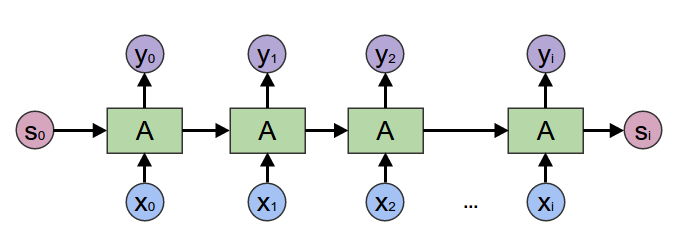
\includegraphics{/img/entries/functional-models/RNN-general.png} {[}colah{]}:
http://colah.github.io/posts/2015-09-NN-Types-FP/

If we look at each one of those individual boxes, they all have two inputs
(normal input, and previous state) and two outputs (normal output, new state).

``Unrolling'' a stateful model means taking a model that takes in an \texttt{X}
and producing a \texttt{Y} and turning it into a model that takes an
\texttt{{[}X{]}} and produces a \texttt{{[}Y{]}}, by feeding it each of the
\texttt{X}s one after the other, propagating the state, and collecting all of
the \texttt{Y} responses.

The ``type'' of this sounds like:

\begin{Shaded}
\begin{Highlighting}[]
\OtherTok{unroll ::} \DataTypeTok{Model}\NormalTok{ p s a b }\OtherTok{->} \DataTypeTok{Model}\NormalTok{ p s [a] [b]}
\end{Highlighting}
\end{Shaded}

In writing this out as a type, we also note that the \texttt{p} parameter type
is the same, and the \texttt{s} state type is the same. (Aren't types nice? They
force you to have to think about subtle things like this) If you're familiar
with category theory, this looks a little bit like a sort of ``fmap'' under a
\texttt{Model\ p\ s} category -- it takes a (stateful and backpropagatable)
\texttt{a\ -\textgreater{}\ b} and turns it into an
\texttt{{[}a{]}\ -\textgreater{}\ {[}b{]}}.

Olah's post suggests that this is some sort of \texttt{mapAccum}, in functional
programming parlance. And, surely enough, we can actually write this as a
\texttt{mapAccumL}.

\texttt{mapAccumL} is sort of like a combination of a \texttt{foldl} and a
\texttt{map}:

\begin{Shaded}
\begin{Highlighting}[]
\NormalTok{mapAccumL}
\OtherTok{    ::}\NormalTok{ (a }\OtherTok{->}\NormalTok{ b }\OtherTok{->}\NormalTok{ (a, c))}
    \OtherTok{->}\NormalTok{ a}
    \OtherTok{->}\NormalTok{ [b]}
    \OtherTok{->}\NormalTok{ (a, [c])}
\end{Highlighting}
\end{Shaded}

Compare to \texttt{foldl}:

\begin{Shaded}
\begin{Highlighting}[]
\NormalTok{foldl}
\OtherTok{    ::}\NormalTok{ (a }\OtherTok{->}\NormalTok{ b }\OtherTok{->}\NormalTok{ a)}
    \OtherTok{->}\NormalTok{ a}
    \OtherTok{->}\NormalTok{ [b]}
    \OtherTok{->}\NormalTok{ a}
\end{Highlighting}
\end{Shaded}

You can see that \texttt{mapAccumL} is just \texttt{foldl}, except the folding
function emits an extra \texttt{c} for every item, so \texttt{mapAccumL} can
return a new \texttt{{[}c{]}} with all of the emitted \texttt{c}s.

The \emph{backprop} library has a ``lifted'' \texttt{mapAccumL} in in the
\emph{\href{http://hackage.haskell.org/package/backprop/docs/Prelude-Backprop.html}{Prelude.Backprop}}
module that we can use:

\begin{Shaded}
\begin{Highlighting}[]
\NormalTok{Prelude.Backprop.mapAccumL}
\OtherTok{    ::}\NormalTok{ (}\DataTypeTok{BVar}\NormalTok{ z a }\OtherTok{->} \DataTypeTok{BVar}\NormalTok{ z b }\OtherTok{->}\NormalTok{ (}\DataTypeTok{BVar}\NormalTok{ z a, }\DataTypeTok{BVar}\NormalTok{ z c))}
    \OtherTok{->} \DataTypeTok{BVar}\NormalTok{ z a}
    \OtherTok{->} \DataTypeTok{BVar}\NormalTok{ z [b]}
    \OtherTok{->}\NormalTok{ (}\DataTypeTok{BVar}\NormalTok{ z a, }\DataTypeTok{BVar}\NormalTok{ z [c])}
\end{Highlighting}
\end{Shaded}

It is lifted to work with \texttt{BVar}s of the items instead of directly on the
items. With that, we can write \texttt{unroll}, which is just a thin wrapper
over \texttt{mapAccumL}:\footnote{In truth, \texttt{mapAccumL} can work with any
  \texttt{Traversable} container, so we really can \texttt{unroll} over any
  \texttt{Traversable} container and not just lists. One of my favorite is the
  sized vectors from the
  \href{http://hackage.haskell.org/package/vector-sized}{vector-sized} library,
  since they can enforce that the network always gets unrolled over the same
  number of items.}

\begin{Shaded}
\begin{Highlighting}[]
\CommentTok{-- source: https://github.com/mstksg/inCode/tree/master/code-samples/functional-models/model.hs#L200-L208}

\NormalTok{unroll}
\OtherTok{    ::}\NormalTok{ (}\DataTypeTok{Backprop}\NormalTok{ a, }\DataTypeTok{Backprop}\NormalTok{ b)}
    \OtherTok{=>} \DataTypeTok{ModelS}\NormalTok{ p s  a   b}
    \OtherTok{->} \DataTypeTok{ModelS}\NormalTok{ p s [a] [b]}
\NormalTok{unroll f p xs s0 }\FunctionTok{=}\NormalTok{ swap }\FunctionTok{$}\NormalTok{ B.mapAccumL f' s0 xs}
  \KeywordTok{where}
    \CommentTok{-- we have to re-arrange the order of arguments and tuple a bit to}
    \CommentTok{-- match what `mapAccumL` expects}
\NormalTok{    f' s x }\FunctionTok{=}\NormalTok{ swap (f p x s)}
\end{Highlighting}
\end{Shaded}

This reveals that \texttt{unroll} from the machine learning is really
\emph{just} \texttt{mapAccumL} from functional programming.

We can also tweak \texttt{unroll}'s result a bit to get a version of
\texttt{unroll} that shows only the ``final'' result. All we do is \texttt{mapS}
\texttt{last\ .\ sequenceVar\ ::\ BVar\ s\ {[}a{]}\ -\textgreater{}\ BVar\ a},
which gets the last item in a \texttt{BVar} of a sequence.

\begin{Shaded}
\begin{Highlighting}[]
\CommentTok{-- source: https://github.com/mstksg/inCode/tree/master/code-samples/functional-models/model.hs#L210-L214}

\NormalTok{unrollLast}
\OtherTok{    ::}\NormalTok{ (}\DataTypeTok{Backprop}\NormalTok{ a, }\DataTypeTok{Backprop}\NormalTok{ b)}
    \OtherTok{=>} \DataTypeTok{ModelS}\NormalTok{ p s  a  b}
    \OtherTok{->} \DataTypeTok{ModelS}\NormalTok{ p s [a] b}
\NormalTok{unrollLast f }\FunctionTok{=}\NormalTok{ mapS (last }\FunctionTok{.}\NormalTok{ sequenceVar) (unroll f)}
\end{Highlighting}
\end{Shaded}

Alternatively, we can also recognize that \texttt{unrollLast} is really just an
awkward left fold (\texttt{foldl}) in disguise:

\begin{Shaded}
\begin{Highlighting}[]
\CommentTok{-- source: https://github.com/mstksg/inCode/tree/master/code-samples/functional-models/model.hs#L216-L222}

\NormalTok{unrollLast'}
\OtherTok{    ::} \DataTypeTok{Backprop}\NormalTok{ a}
    \OtherTok{=>} \DataTypeTok{ModelS}\NormalTok{ p s  a  b}
    \OtherTok{->} \DataTypeTok{ModelS}\NormalTok{ p s [a] b}
\NormalTok{unrollLast' f p xs s0 }\FunctionTok{=}\NormalTok{ foldl' go (undefined, s0) (sequenceVar xs)}
  \KeywordTok{where}
\NormalTok{    go (_, s) x }\FunctionTok{=}\NormalTok{ f p x s}
\end{Highlighting}
\end{Shaded}

To see how this applies to our \texttt{threeLayer}:

\begin{Shaded}
\begin{Highlighting}[]
\OtherTok{threeLayers            ::} \DataTypeTok{ModelS}\NormalTok{ _ _ (}\DataTypeTok{R} \DecValTok{40}\NormalTok{) (}\DataTypeTok{R} \DecValTok{5}\NormalTok{)}
\NormalTok{unroll}\OtherTok{     threeLayers ::} \DataTypeTok{ModelS}\NormalTok{ _ _ [}\DataTypeTok{R} \DecValTok{40}\NormalTok{] [}\DataTypeTok{R} \DecValTok{5}\NormalTok{]}
\NormalTok{unrollLast}\OtherTok{ threeLayers ::} \DataTypeTok{ModelS}\NormalTok{ _ _ [}\DataTypeTok{R} \DecValTok{40}\NormalTok{] (}\DataTypeTok{R} \DecValTok{5}\NormalTok{)}
\end{Highlighting}
\end{Shaded}

Nice that we can trace the evolution of the types within our langage!

\hypertarget{state-be-gone}{%
\subsection{State-be-gone}\label{state-be-gone}}

Did you enjoy the detour through stateful time series models?

Good --- because the whole point of it was to talk about how we can \emph{get
rid of state} and bring us back to our original models!

You knew this day had to come, because all of our methods for ``training'' these
models and learn these parameters involves non-stateful models. Let's see now
how we can turn our functional stateful models into functional non-stateful
models!

One way is to \emph{fix the initial state and throw away the resulting one}.
This is very common in machine learning contexts, where many people simply fix
the initial state to be a zero vector.

\begin{Shaded}
\begin{Highlighting}[]
\CommentTok{-- source: https://github.com/mstksg/inCode/tree/master/code-samples/functional-models/model.hs#L225-L235}

\NormalTok{fixState}
\OtherTok{    ::}\NormalTok{ s}
    \OtherTok{->} \DataTypeTok{ModelS}\NormalTok{ p s a b}
    \OtherTok{->} \DataTypeTok{Model}\NormalTok{  p   a b}
\NormalTok{fixState s0 f p x }\FunctionTok{=}\NormalTok{ fst }\FunctionTok{$}\NormalTok{ f p x (auto s0)}

\NormalTok{zeroState}
\OtherTok{    ::} \DataTypeTok{Num}\NormalTok{ s}
    \OtherTok{=>} \DataTypeTok{ModelS}\NormalTok{ p s a b}
    \OtherTok{->} \DataTypeTok{Model}\NormalTok{  p   a b}
\NormalTok{zeroState }\FunctionTok{=}\NormalTok{ fixState }\DecValTok{0}
\end{Highlighting}
\end{Shaded}

We use \texttt{auto\ ::\ a\ -\textgreater{}\ BVar\ z\ a} again to introduce a
\texttt{BVar} of our initial state, but to indicate that we don't expect to
track its gradient. \texttt{zeroState} is a nice utility combinator for a common
pattern.

Another way is to \emph{treat the initial state as a trainable parameter} (and
also throw away the final state). This is not done as often, but is still common
enough to be mentioned often. And, it's just as straightforward!

\begin{Shaded}
\begin{Highlighting}[]
\CommentTok{-- source: https://github.com/mstksg/inCode/tree/master/code-samples/functional-models/model.hs#L237-L241}

\NormalTok{trainState}
\OtherTok{    ::}\NormalTok{ (}\DataTypeTok{Backprop}\NormalTok{ p, }\DataTypeTok{Backprop}\NormalTok{ s)}
    \OtherTok{=>} \DataTypeTok{ModelS}\NormalTok{  p    s  a b}
    \OtherTok{->} \DataTypeTok{Model}\NormalTok{  (p }\FunctionTok{:&}\NormalTok{ s) a b}
\NormalTok{trainState f (p }\FunctionTok{:&&}\NormalTok{ s) x }\FunctionTok{=}\NormalTok{ fst }\FunctionTok{$}\NormalTok{ f p x s}
\end{Highlighting}
\end{Shaded}

\texttt{trainState} will take a model with trainable parameter \texttt{p} and
state \texttt{s}, and turn it into a model with trainable parameter
\texttt{p\ :\&\ s}, where the \texttt{s} is the (trainable) initial state.

We can now \emph{train} our recurrent/stateful models, by \textbf{unrolling and
de-stating}:

\begin{Shaded}
\begin{Highlighting}[]
\OtherTok{threeLayers                        ::} \DataTypeTok{ModelS}\NormalTok{ _ _ (}\DataTypeTok{R} \DecValTok{40}\NormalTok{) (}\DataTypeTok{R} \DecValTok{5}\NormalTok{)}
\NormalTok{unrollLast}\OtherTok{ threeLayers             ::} \DataTypeTok{ModelS}\NormalTok{ _ _ [}\DataTypeTok{R} \DecValTok{40}\NormalTok{] (}\DataTypeTok{R} \DecValTok{5}\NormalTok{)}
\NormalTok{zeroState (unrollLast threeLayers)}\OtherTok{ ::} \DataTypeTok{Model}\NormalTok{  _   [}\DataTypeTok{R} \DecValTok{40}\NormalTok{] (}\DataTypeTok{R} \DecValTok{5}\NormalTok{)}
\end{Highlighting}
\end{Shaded}

\texttt{zeroState\ (unrollLast\ threeLayers)} is now a normal stateless (and
trainable) model. It takes a list of inputs \texttt{R\ 40}s and produces the
``final output'' \texttt{R\ 5}. We can now train this by feeding it with
\texttt{({[}R\ 40{]},\ R\ 5)} pairs: give a history and an expected next output.

It's again nice here how we can track the evolution of the types of out model's
inputs and outputs within the language. Unrolling and zeroing is a non-trivial
interaction, so the ability to have the language and compiler track the
resulting shapes of our models is a huge advantage.

\hypertarget{the-unreasonably-effective}{%
\subsection{The Unreasonably Effective}\label{the-unreasonably-effective}}

Let's see if we can train a two-layer fully connected neural network with 30
hidden units, where the first layer is fully recurrent, to learn how to model a
sine wave:

\begin{Shaded}
\begin{Highlighting}[]
\CommentTok{-- sine signal with period 25}
\NormalTok{ghci}\FunctionTok{>}\NormalTok{ series }\FunctionTok{=}\NormalTok{ [ sin (}\DecValTok{2} \FunctionTok{*}\NormalTok{ pi }\FunctionTok{*}\NormalTok{ t }\FunctionTok{/} \DecValTok{25}\NormalTok{) }\FunctionTok{|}\NormalTok{ t }\OtherTok{<-}\NormalTok{ [}\DecValTok{0}\FunctionTok{..}\NormalTok{]              ]}

\CommentTok{-- chunks of runs and "next results"}
\NormalTok{ghci}\FunctionTok{>}\NormalTok{ samps  }\FunctionTok{=}\NormalTok{ [ (init c, last c)      }\FunctionTok{|}\NormalTok{ c }\OtherTok{<-}\NormalTok{ chunksOf }\DecValTok{19}\NormalTok{ series ]}

\CommentTok{-- first layer is RNN, second layer is normal ANN, 30 hidden units}
\NormalTok{ghci}\FunctionTok{>} \KeywordTok{let}\OtherTok{ rnn ::} \DataTypeTok{ModelS}\NormalTok{ _ _ (}\DataTypeTok{R} \DecValTok{1}\NormalTok{) (}\DataTypeTok{R} \DecValTok{1}\NormalTok{)}
\NormalTok{          rnn }\FunctionTok{=}\NormalTok{ feedForward }\FunctionTok{@}\DecValTok{30} \FunctionTok{@}\DecValTok{1} \FunctionTok{<*~}\NormalTok{ mapS logistic (fcrnn }\FunctionTok{@}\DecValTok{1} \FunctionTok{@}\DecValTok{30}\NormalTok{)}

\NormalTok{ghci}\FunctionTok{>}\NormalTok{ trained }\OtherTok{<-}\NormalTok{ trainModelIO (zeroState (unrollLast rnn)) }\FunctionTok{$}\NormalTok{ take }\DecValTok{10000}\NormalTok{ samps}
\end{Highlighting}
\end{Shaded}

Trained! \texttt{trained} is now the weight and bias matrices and vectors that
will simulate a sine wave of period 25.

We can run this model iteratively upon itself to test it; if we plot the
results, we can visually inspect it to see if it has learned things properly.

Let's define some helper functions to test our model. First, a function
\texttt{prime} that takes a stateful model and gives a ``warmed-up'' state by
running it over a list of inputs. This serves to essentially initialize the
memory of the model.

\begin{Shaded}
\begin{Highlighting}[]
\CommentTok{-- source: https://github.com/mstksg/inCode/tree/master/code-samples/functional-models/model.hs#L243-L250}

\NormalTok{prime}
\OtherTok{    ::} \DataTypeTok{Foldable}\NormalTok{ t}
    \OtherTok{=>} \DataTypeTok{ModelS}\NormalTok{ p s a b     }\CommentTok{-- ^ model}
    \OtherTok{->}\NormalTok{ p                  }\CommentTok{-- ^ parameterization}
    \OtherTok{->}\NormalTok{ s                  }\CommentTok{-- ^ initial state}
    \OtherTok{->}\NormalTok{ t a                }\CommentTok{-- ^ priming input}
    \OtherTok{->}\NormalTok{ s                  }\CommentTok{-- ^ primed state}
\NormalTok{prime f p }\FunctionTok{=}\NormalTok{ foldl' }\FunctionTok{$}\NormalTok{ evalBP2 (\textbackslash{}s x }\OtherTok{->}\NormalTok{ snd }\FunctionTok{$}\NormalTok{ f (auto p) x s)}
\end{Highlighting}
\end{Shaded}

Then a function \texttt{feedback} that iterates a stateful model over and over
again by feeding its previous output as its next input:

\begin{Shaded}
\begin{Highlighting}[]
\CommentTok{-- source: https://github.com/mstksg/inCode/tree/master/code-samples/functional-models/model.hs#L252-L263}

\NormalTok{feedback}
\OtherTok{    ::}\NormalTok{ (}\DataTypeTok{Backprop}\NormalTok{ a, }\DataTypeTok{Backprop}\NormalTok{ s)}
    \OtherTok{=>} \DataTypeTok{ModelS}\NormalTok{ p s a a     }\CommentTok{-- ^ model}
    \OtherTok{->}\NormalTok{ p                  }\CommentTok{-- ^ parameterization}
    \OtherTok{->}\NormalTok{ s                  }\CommentTok{-- ^ initial state}
    \OtherTok{->}\NormalTok{ a                  }\CommentTok{-- ^ initial input}
    \OtherTok{->}\NormalTok{ [a]                }\CommentTok{-- ^ inifinite feedback loop}
\NormalTok{feedback f p s0 x0 }\FunctionTok{=}\NormalTok{ unfoldr go (x0, s0)}
  \KeywordTok{where}
\NormalTok{    go (x, s) }\FunctionTok{=} \DataTypeTok{Just}\NormalTok{ (x, (y, s'))}
      \KeywordTok{where}
\NormalTok{        (y, s') }\FunctionTok{=}\NormalTok{ evalBP (uncurry }\DataTypeTok{T2} \FunctionTok{.}\NormalTok{ f (auto p) (auto x)) s}
\end{Highlighting}
\end{Shaded}

Now let's prime our trained model over the first 19 items in our sine wave and
start it running in feedback mode on the 20th item!

\begin{Shaded}
\begin{Highlighting}[]
\NormalTok{ghci}\FunctionTok{>} \KeywordTok{let}\NormalTok{ primed }\FunctionTok{=}\NormalTok{ prime    rnn trained }\DecValTok{0}\NormalTok{      (take }\DecValTok{19}\NormalTok{ series)}
\NormalTok{ghci}\FunctionTok{>} \KeywordTok{let}\NormalTok{ output }\FunctionTok{=}\NormalTok{ feedback rnn trained primed (series }\FunctionTok{!!} \DecValTok{19}\NormalTok{)}
\NormalTok{ghci}\FunctionTok{>}\NormalTok{ mapM_ print }\FunctionTok{$}\NormalTok{ take }\DecValTok{200}\NormalTok{ output}
\NormalTok{(}\FunctionTok{-}\FloatTok{0.9980267284282716}\OtherTok{ ::} \DataTypeTok{R} \DecValTok{1}\NormalTok{)}
\NormalTok{(}\FunctionTok{-}\FloatTok{0.9530599469923343}\OtherTok{ ::} \DataTypeTok{R} \DecValTok{1}\NormalTok{)}
\NormalTok{(}\FunctionTok{-}\FloatTok{0.855333250123637}\OtherTok{ ::} \DataTypeTok{R} \DecValTok{1}\NormalTok{)}
\NormalTok{(}\FunctionTok{-}\FloatTok{0.7138776465246676}\OtherTok{ ::} \DataTypeTok{R} \DecValTok{1}\NormalTok{)}
\NormalTok{(}\FunctionTok{-}\FloatTok{0.5359655931506458}\OtherTok{ ::} \DataTypeTok{R} \DecValTok{1}\NormalTok{)}
\CommentTok{-- ...}
\end{Highlighting}
\end{Shaded}

Plotting the result against the ``actual'' sine wave of period 25, we see that
it approximates the process decently well, with a consistent period (that is
slightly slower than the reference period):

\begin{figure}
\centering
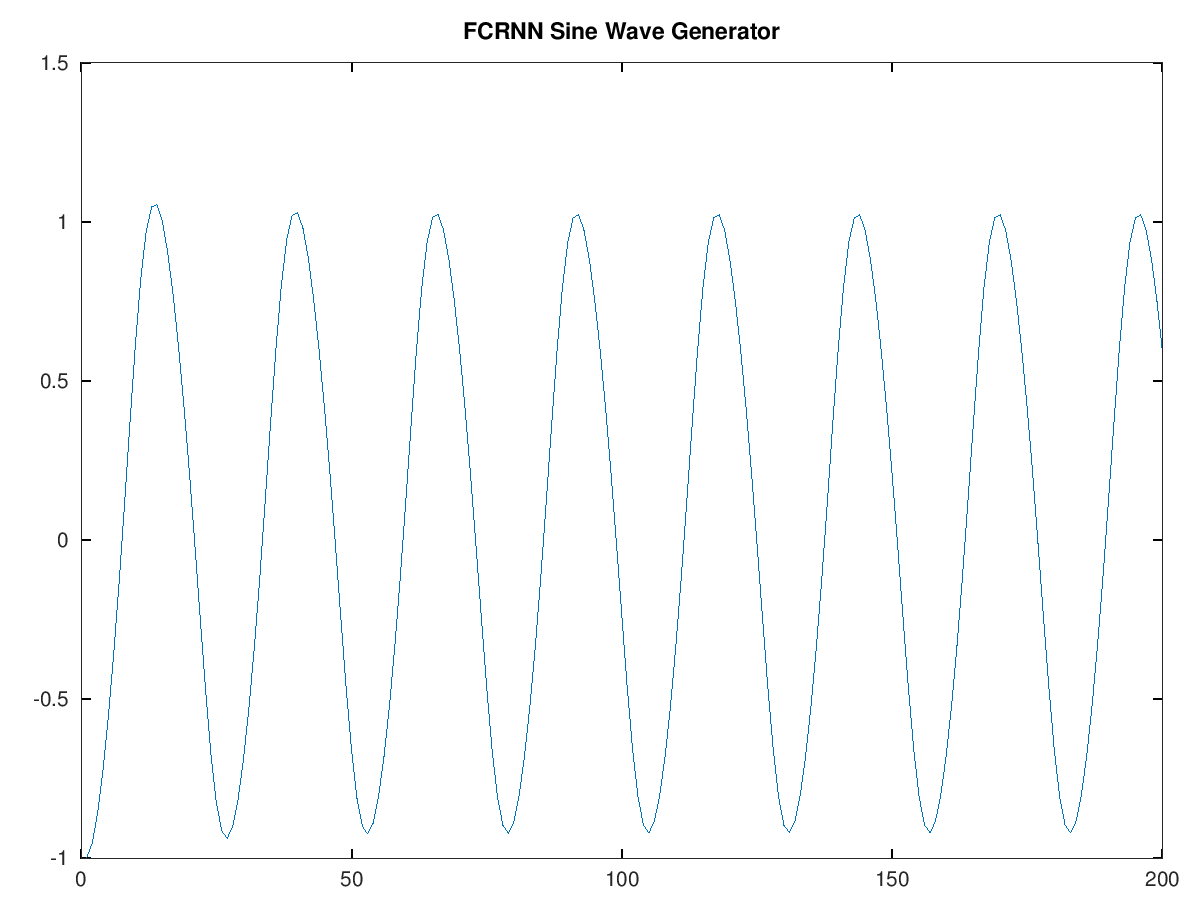
\includegraphics{/img/entries/functional-models/rnnsin.png}
\caption{FCRNN Sine Wave}
\end{figure}

For kicks, let's see if we can do any better with the simpler AR(2) model from
before. Applying all we just used to \texttt{ar2}, we see:

\begin{Shaded}
\begin{Highlighting}[]
\OtherTok{ar2                        ::} \DataTypeTok{ModelS}\NormalTok{ _ _  }\DataTypeTok{Double}  \DataTypeTok{Double}
\NormalTok{unrollLast}\OtherTok{ ar2             ::} \DataTypeTok{ModelS}\NormalTok{ _ _ [}\DataTypeTok{Double}\NormalTok{] }\DataTypeTok{Double}
\NormalTok{zeroState (unrollLast ar2)}\OtherTok{ ::} \DataTypeTok{Model}\NormalTok{  _   [}\DataTypeTok{Double}\NormalTok{] }\DataTypeTok{Double}
\end{Highlighting}
\end{Shaded}

\texttt{zeroState\ (unrollLast\ ar2)} is now a trainable stateless model. Will
it model a sine wave?

\begin{Shaded}
\begin{Highlighting}[]
\NormalTok{ghci}\FunctionTok{>}\NormalTok{ trained }\OtherTok{<-}\NormalTok{ trainModelIO (zeroState (unrollLast ar2)) }\FunctionTok{$}\NormalTok{ take }\DecValTok{10000}\NormalTok{ samps}
\NormalTok{ghci}\FunctionTok{>} \KeywordTok{let}\NormalTok{ primed }\FunctionTok{=}\NormalTok{ prime    rnn trained }\DecValTok{0}\NormalTok{      (take }\DecValTok{19}\NormalTok{ series)}
\NormalTok{ghci}\FunctionTok{>} \KeywordTok{let}\NormalTok{ output }\FunctionTok{=}\NormalTok{ feedback rnn trained primed (series }\FunctionTok{!!} \DecValTok{19}\NormalTok{)}
\NormalTok{ghci}\FunctionTok{>}\NormalTok{ mapM_ print }\FunctionTok{$}\NormalTok{ take }\DecValTok{200}\NormalTok{ output}
\NormalTok{(}\FunctionTok{-}\FloatTok{0.9980267284282716}\OtherTok{ ::} \DataTypeTok{R} \DecValTok{1}\NormalTok{)}
\NormalTok{(}\FunctionTok{-}\FloatTok{0.9530599469923343}\OtherTok{ ::} \DataTypeTok{R} \DecValTok{1}\NormalTok{)}
\NormalTok{(}\FunctionTok{-}\FloatTok{0.855333250123637}\OtherTok{ ::} \DataTypeTok{R} \DecValTok{1}\NormalTok{)}
\NormalTok{(}\FunctionTok{-}\FloatTok{0.7138776465246676}\OtherTok{ ::} \DataTypeTok{R} \DecValTok{1}\NormalTok{)}
\NormalTok{(}\FunctionTok{-}\FloatTok{0.5359655931506458}\OtherTok{ ::} \DataTypeTok{R} \DecValTok{1}\NormalTok{)}
\CommentTok{-- ...}
\end{Highlighting}
\end{Shaded}

We can plot the result and see that it more or less perfectly models the sine
wave of period 25:

\begin{figure}
\centering
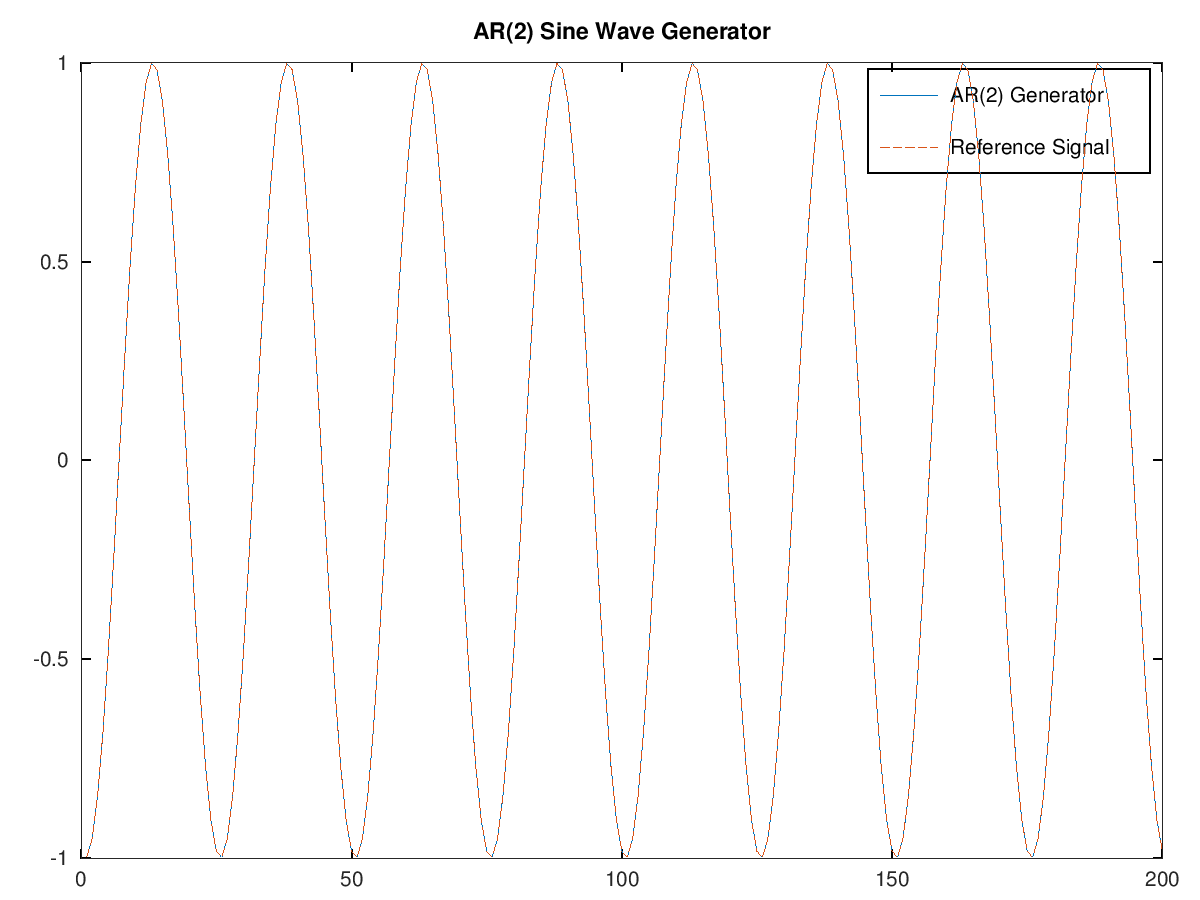
\includegraphics{/img/entries/functional-models/ar2sin.png}
\caption{AR(2) Sine Wave}
\end{figure}

You can't even visually see the difference!

We can peek inside the parameterization of our learned AR(2):

\begin{Shaded}
\begin{Highlighting}[]
\NormalTok{ghci}\FunctionTok{>}\NormalTok{ trained}
\FunctionTok{-}\FloatTok{2.4013298985824788e-12} \FunctionTok{:&}\NormalTok{ (}\FloatTok{1.937166322256747} \FunctionTok{:&} \FunctionTok{-}\FloatTok{0.9999999999997953}\NormalTok{)}
\CommentTok{-- approximately}
\FloatTok{0.0000} \FunctionTok{:&}\NormalTok{ (}\FloatTok{1.9372} \FunctionTok{:&} \FunctionTok{-}\FloatTok{1.0000}\NormalTok{)}
\end{Highlighting}
\end{Shaded}

Meaning that the gradient descent has concluded that our AR(2) model is:

{[} y\_t = 0 + 1.9372 y\_\{t - 1\} - y\_\{t -
2\}{]}(https://latex.codecogs.com/png.latex?\%0Ay\_t\%20\%3D\%200\%20\%2B\%201.9372\%20y\_\%7Bt\%20-\%201\%7D\%20-\%20y\_\%7Bt\%20-\%202\%7D\%0A
" y\_t = 0 + 1.9372 y\_\{t - 1\} - y\_\{t - 2\} ``)

The power of math!

In this toy situation, the AR(2) appears to do much better than our RNN model,
but we have to give the RNN a break --- all of the information has to be
``squished'' into essentially 30 bits, which might impact the model's accuracy.

\hypertarget{functions-all-the-way-down}{%
\section{Functions all the way down}\label{functions-all-the-way-down}}

Again, it is very easy to look at something like

\begin{Shaded}
\begin{Highlighting}[]
\NormalTok{feedForward }\FunctionTok{@}\DecValTok{10} \FunctionTok{<*~}\NormalTok{ mapS logistic fcrnn}
\end{Highlighting}
\end{Shaded}

and write it off as some abstract API of opaque data types. Some sort of object
keeps track of state, and the object has some nice abstracted
interface\ldots{}right?

But, nope, again, it is all just normal functions that we wrote using normal
function composition. We define our model as a \emph{function}, and the backprop
library turns that function into a trainable model.

\hypertarget{what-makes-it-tick}{%
\subsection{What Makes It Tick}\label{what-makes-it-tick}}

Let's again revisit the four things I mentioned that are essential to making
this all work at the end of the last post, but update it with new observations
that we made in this post:

\begin{enumerate}
\def\labelenumi{\arabic{enumi}.}
\item
  \emph{Functional programming} is the paradigm that allowed us to treat
  everything as normal functions, so that our combinators are all just normal
  higher-order functions.

  Our stateful models can also be combined and reshaped seamlessly in arbitrary
  ways, just like our non-stateful ones. And the fact that they are both normal
  functions means that they are built on the same underlying mechanic.

  We can \emph{write} combinators like \texttt{(\textless{}*\textasciitilde{}*)}
  and \texttt{mapS}, but they are never \emph{necessary}. They are always just
  \emph{convenient}. But by writing such combinators, we open our mind to
  different ways that we can construct new models by simply transforming old
  ones.

  The revelation that an unrolled model was simply a combinator application came
  about by simply looking at the types and applying a model to a simple higher
  order function \texttt{mapAccumL} and \texttt{foldl}, which was \emph{already
  written for us}. We were able to use \emph{common functional programming
  tools} that are provided in standard libraries. This is only possible because
  our models are themselves functions in the same shape that those common tools
  already are built to work on.

  In addition, functional programming forces us to have \emph{first-class
  state}. The ``state'' in our stateful models wasn't a property of the runtime
  system --- they were things we explicitly defined and carried. This allows us
  to write combinators that \emph{manipulate how state works}. We can transform
  a function's state arbitrarily because the function's state is always
  something we can explicitly manipulate.
\item
  \emph{Differentiable} programs --- again, made more powerful through how well
  it integrates with functional programming techniques.
\item
  \emph{Purely} functional programming. One might have thought that writing
  ``recurrent'' or ``stateful'' models were something that imperative models
  excelled in, but we see now that in a functional setting, forcing ourselves to
  use explicit state allows us to manipulate state and state manipulation as a
  first-class citizen of our language, instead of something built-in and
  implicit and rigid.
\item
  A \emph{strong expressive static type system} ties all of this together and
  makes it possible to work in.

  This forces us to be aware of what parameters we have, how they combine, etc.;
  this is what makes combinators like \texttt{recurrent} and \texttt{unroll} and
  \texttt{zeroState} reasonable: the \emph{compiler} is able to trace how we
  move around our parameter and state, so that we don't have to. It lets us ask
  \emph{the compiler} questions like ``what is the state type, now?'' if we
  needed, or ``what is the parameter type now?''.

  We sometimes even gained insight simply from thinking, in advance, what the
  types of our combinators were. We had to make conscious decisions when writing
  the type of \texttt{unroll} and \texttt{zeroState}. And, if we can phrase our
  combinators in terms of our types, the compiler will often be able to write
  our entire program for us --- something only possible for statically typed
  languages.
\end{enumerate}

In the next and final post, we'll wrap this up by peeking into the wonderful
world of functional combinators and look at powerful ones that allow us to unify
many different model types as really just different combinator applications of
the same thing. I'll also talk about what I think are essential in building a
usable framework for working with this in practice.

\end{document}
